\begin{center}
\footnotesize\noindent\fbox{
	\parbox{\textwidth}{
	Con riferimento al sistema lineare dell'Esercizio 3, con $n=1000$, graficare la norma dei residui rispetto all'indice di iterazione, generati dai metodi di Jacobi e Gauss-Seidel. Utilizzare il formato \lstinline[language=Matlab]{semilogy} per realizzare il grafico, corredandolo di opportune $label$.
} }
\end{center}

\noindent Il grafico seguente \'e quello richiesto, realizzato con le ascisse in scala logaritmica tramite il formato semilogaritmico \lstinline[language=Matlab]{semilogy} di Matlab.

\begin{center}
	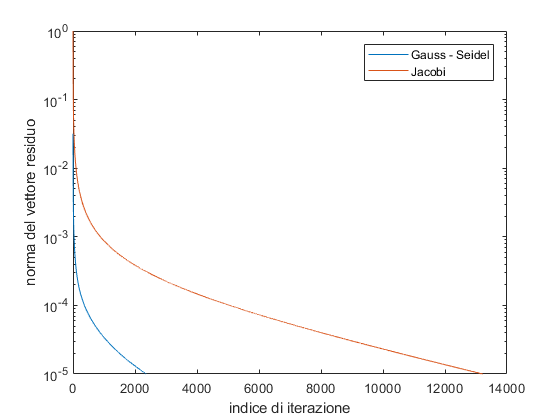
\includegraphics[scale=0.9]{cap6/6_5.png}
\end{center}

\noindent Il codice Matlab utilizzato per la sua realizzazione \'e quello che segue. Si noti che sono state modificate le function degli esercizi precedenti in modo da memorizzare la norma dei residui di ogni iterazione in un vettore, poi restituito in output.

\lstinputlisting[language=Matlab]{cap6/6_5.m}
